\chapter{工作概况}

非固定文本填写区域

\section{技术服务工作情况}

\subsection{建档情况}

广东省深圳市10个地区在2015年1月1日至2015年12月31日期间,共创建家庭档案34457份,其中评估完成档案34281份,评估未完成档案176份,评估完成率为99.49\%。2015年度各地区建档及评估完成情况如图\ref{图1}所示。
\begin{figure}[htbp]
	\centering
	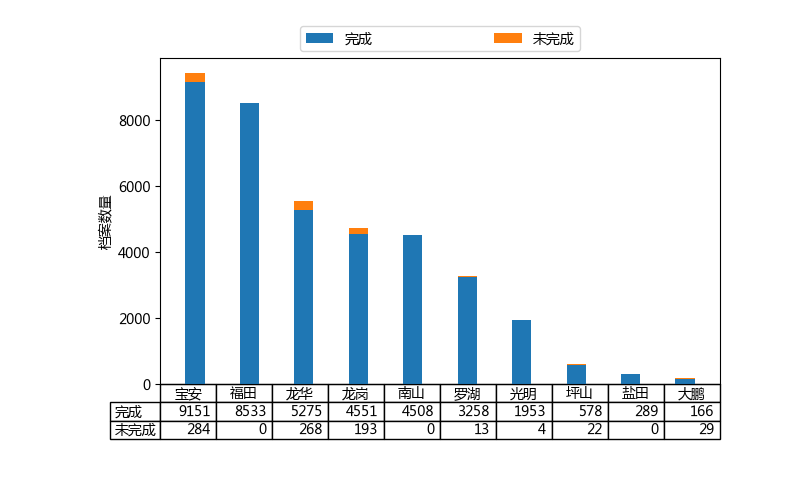
\includegraphics[width=1\textwidth]{1.png}
	\caption{2015年广东省深圳市各地区建档及完成情况}
	\label{图1}
\end{figure}




在2015年度广东省深圳市参加检查的服务对象中,夫妻双方共同参加检查的档案占档案总数的96.66\%,女方单独参加检查的档案占档案总数的2.71\%,男方单独参加检查的档案占档案总数的0.63\%。2015年度各地区知情同意书签署情况如图\ref{图2}所示。
\begin{figure}[htbp]
	\centering
	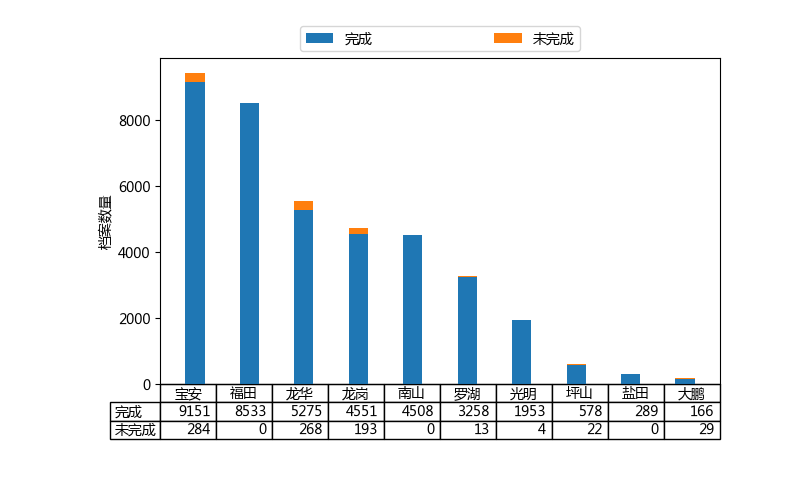
\includegraphics[width=1\textwidth]{1.png}
	\caption{测试图片}
	\label{图2}
\end{figure}


 

\subsection{检查人数}

广东省深圳市10个地区在2015年1月1日至2015年12月31日期间共有67762人参加检查,其中男性有33523人,女性有45594人。2015年度各地区参加检查的人数情况如图\ref{图3}所示。
\begin{figure}[htbp]
	\centering
	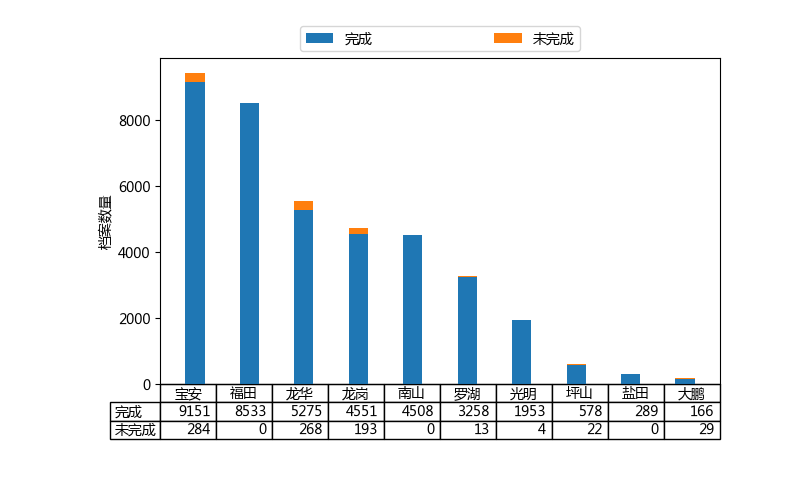
\includegraphics[width=1\textwidth]{1.png}
	\caption{测试图片}
	\label{图3}
\end{figure}




\subsection{风险评估情况}

2015年广东省深圳市10个地区共完成评估的档案为34281份。评估为一般人群的档案占评估总档案的73.17\%,评估为风险人群的档案占评估总档案的26.86\%,其中评估为男性单方风险的人群占评估总档案的3.88\%,女性单方风险的人群占评估总档案的8.74\%,双方风险的人群占评估总档案的14.24。2015年广东省深圳市风险人群评估比例构成风险人群评估比例如下图所示。



\subsection{计划怀孕二胎比例}

2015年度参加孕前检查并完成风险评估的女性中,计划生育头胎、二胎及三胎以上者分别占参检女性的19.22\%、79.78\%、和1.00\%。与2014年度参检女性计划怀孕二胎的比例(85.23\%)相比有明显上升,表明国家全面两孩政策实施以后广东省深圳市参加孕前检查的服务对象中计划生二胎的比例已上升至一半以上。广东省深圳市各地区计划怀孕的胎次构成情况如下图所示。



\section{随访管理工作情况}

\subsection{早孕随访情况}

2015年1月1日至2015年12月31日(以早孕随访日期来统计),广东省深圳市10个地区共做了10839人次早孕随访,已经完成的早孕随访档案有10839份,其中早孕随访结果为失访的档案有894份,占早孕随访完成档案的14.28\%。未完成的早孕随访档案有0份,其中有None\%的早孕随访结果是未孕。2015年广东省深圳市各地区已完成早孕随访的情况如下图所示。



\subsection{妊娠结局随访情况}

2015年1月1日至2015年12月31日(以妊娠结局随访日期来统计),广东省深圳市10个地区共做了8759人次妊娠结局随访,已经完成的妊娠结局随访档案有8759份,其中妊娠结局随访结果为失访的档案有310份,占妊娠结局随访完成档案的3.54\%。未完成的妊娠结局随访档案有0份,其中有None\%的妊娠结局随访结果是未分娩。2015年广东省深圳市各地区已完成妊娠结局随访的情况如下图所示。



\subsection{参检人群1年妊娠率}

为间接反映广东省深圳市国家免费孕前优生健康检查项目目标人群入选的准确性,利用2014年度和2015年度的全国数据,以风险评估日期在2014年1月-12月范围内的待孕参检家庭总数为分母,参检后成功受孕且末次月经与参检日期间隔在-1月至12个月内的参检家庭数为分子,计算孕前项目参加家庭1年妊娠率。截至2015年12月31日,广东省深圳市参检家庭1年妊娠率平均为12.64\%,比上一年度的8.65\%有显著提高。2015年度和2014年度广东省深圳市各地区参检人群1年妊娠率的情况如下图所示。



\subsection{不良结局统计}

在完成妊娠结局随访的档案中,正常活产有7682例,占87.70\%,不良妊娠结局占12.30\%。在所有的不良妊娠结局中,排名前三位(待修改:支持排序)的是自然流产(4.58\%)、低出生体重(2.54\%)和医学性人工流产(2.30\%)。【名称为:(natrualpre, lower\_weight, medicinepre, bornfault, earlypre, treatpre, differentpre, deathpre, qitapre); [(1, 0, 0, 0, 0, 0, 0, 0, None), (0, 1, 0, 0, 0, 0, 0, 0, None), (0, 0, 1, 0, 0, 0, 0, 0, None)],数值为3.47\%、2.19\%、1.99\%】。2015年广东省深圳市妊娠结局的构成以及不良妊娠结局的构成如下图所示。





